\documentclass[a4paper,12pt]{article}

\usepackage[T2A]{fontenc}			
\usepackage[utf8]{inputenc}			
\usepackage[english,russian]{babel}	

\usepackage[
bookmarks=true, colorlinks=true, unicode=true,
urlcolor=black,linkcolor=black, anchorcolor=black,
citecolor=black, menucolor=black, filecolor=black,
]{hyperref}

\usepackage{color}
\usepackage{caption}
\DeclareCaptionFont{white}{\color{black}}
\DeclareCaptionFormat{listing}{\colorbox{white}{\parbox{\textwidth}{#1#2#3}}}
\captionsetup[lstlisting]{format=listing,labelfont=white,textfont=white}

\usepackage{amsmath,amsfonts,amssymb,amsthm,mathtools} 
\usepackage{wasysym}

\usepackage{graphicx}
%\usepackage[cache=false]{minted}
\usepackage{cmap}
\usepackage{indentfirst}

\usepackage{listings} 
\usepackage{fancyvrb}

\usepackage{geometry}
\geometry{left=2cm}
\geometry{right=1.5cm}
\geometry{top=1cm}
\geometry{bottom=2cm}

\setlength{\parindent}{5ex}
\setlength{\parskip}{0.5em}

\usepackage{pgfplots}
\usetikzlibrary{datavisualization}
\usetikzlibrary{datavisualization.formats.functions}

\begin{document}
	\lstset{ %
		language=C,                 % выбор языка для подсветки (здесь это С)
		basicstyle=\small\sffamily, % размер и начертание шрифта для подсветки кода
		numbers=left,               % где поставить нумерацию строк (слева\справа)
		numberstyle=\tiny,           % размер шрифта для номеров строк
		stepnumber=1,                   % размер шага между двумя номерами строк
		numbersep=5pt,                % как далеко отстоят номера строк от подсвечиваемого кода
		backgroundcolor=\color{white}, % цвет фона подсветки - используем \usepackage{color}
		showspaces=false,            % показывать или нет пробелы специальными отступами
		showstringspaces=false,      % показывать или нет пробелы в строках
		showtabs=false,             % показывать или нет табуляцию в строках
		frame=single,              % рисовать рамку вокруг кода
		tabsize=2,                 % размер табуляции по умолчанию равен 2 пробелам
		captionpos=t,              % позиция заголовка вверху [t] или внизу [b] 
		breaklines=true,           % автоматически переносить строки (да\нет)
		breakatwhitespace=false, % переносить строки только если есть пробел
		escapeinside={\%*}{*)}   % если нужно добавить комментарии в коде
	}
	
	% Титульный лист
	\begin{figure}[h!]
		\begin{center}
			{
\includegraphics[scale = 0.4]{titul.jpg}}
			\label{titul}
		\end{center}
	\end{figure}
	
	\vspace*{15mm} 
	
	\huge
	\begin{center}
		Дисциплина: <<Операционные системы>>
	\end{center}
	
	\begin{center}
		Лабораторная работа №6
	\end{center}

	
	\huge
	\begin{center}
		Тема работы:\\
		<<Сокеты>>
	\end{center}
	\vspace*{30mm} 
	
	\large
	\begin{flushright}
		Студент: Левушкин И. К. \\
		Группа: ИУ7-62Б \\
		Преподаватель: Рязанова Н. Ю. \\
	\end{flushright}
	
	\vspace*{30mm}
	\begin{center}
		Москва, 2020 г.  
	\end{center}
	\thispagestyle{empty}
	
	
	\newpage
	
	\section*{Задание 1.}
	
	{\bf Написать приложение по модели клиент-сервер, демонстрирующее взаимодействие параллельных процессов на отдельном компьютере с использованием сокетов в файловом пространстве имен: семейство - AF\_UNIX, тип - SOCK\_DGRAM. При демонстрации работы программного комплекса необходимо запустить несколько клиентов (не меньше 5) и продемонстрировать, что сервер обрабатывает обращения каждого запущенного клиента.}
	
	Ниже приведен программный комплекс, реализующий поставленную задачу.
	
	\begin{figure}[h!]
		\begin{center}
			{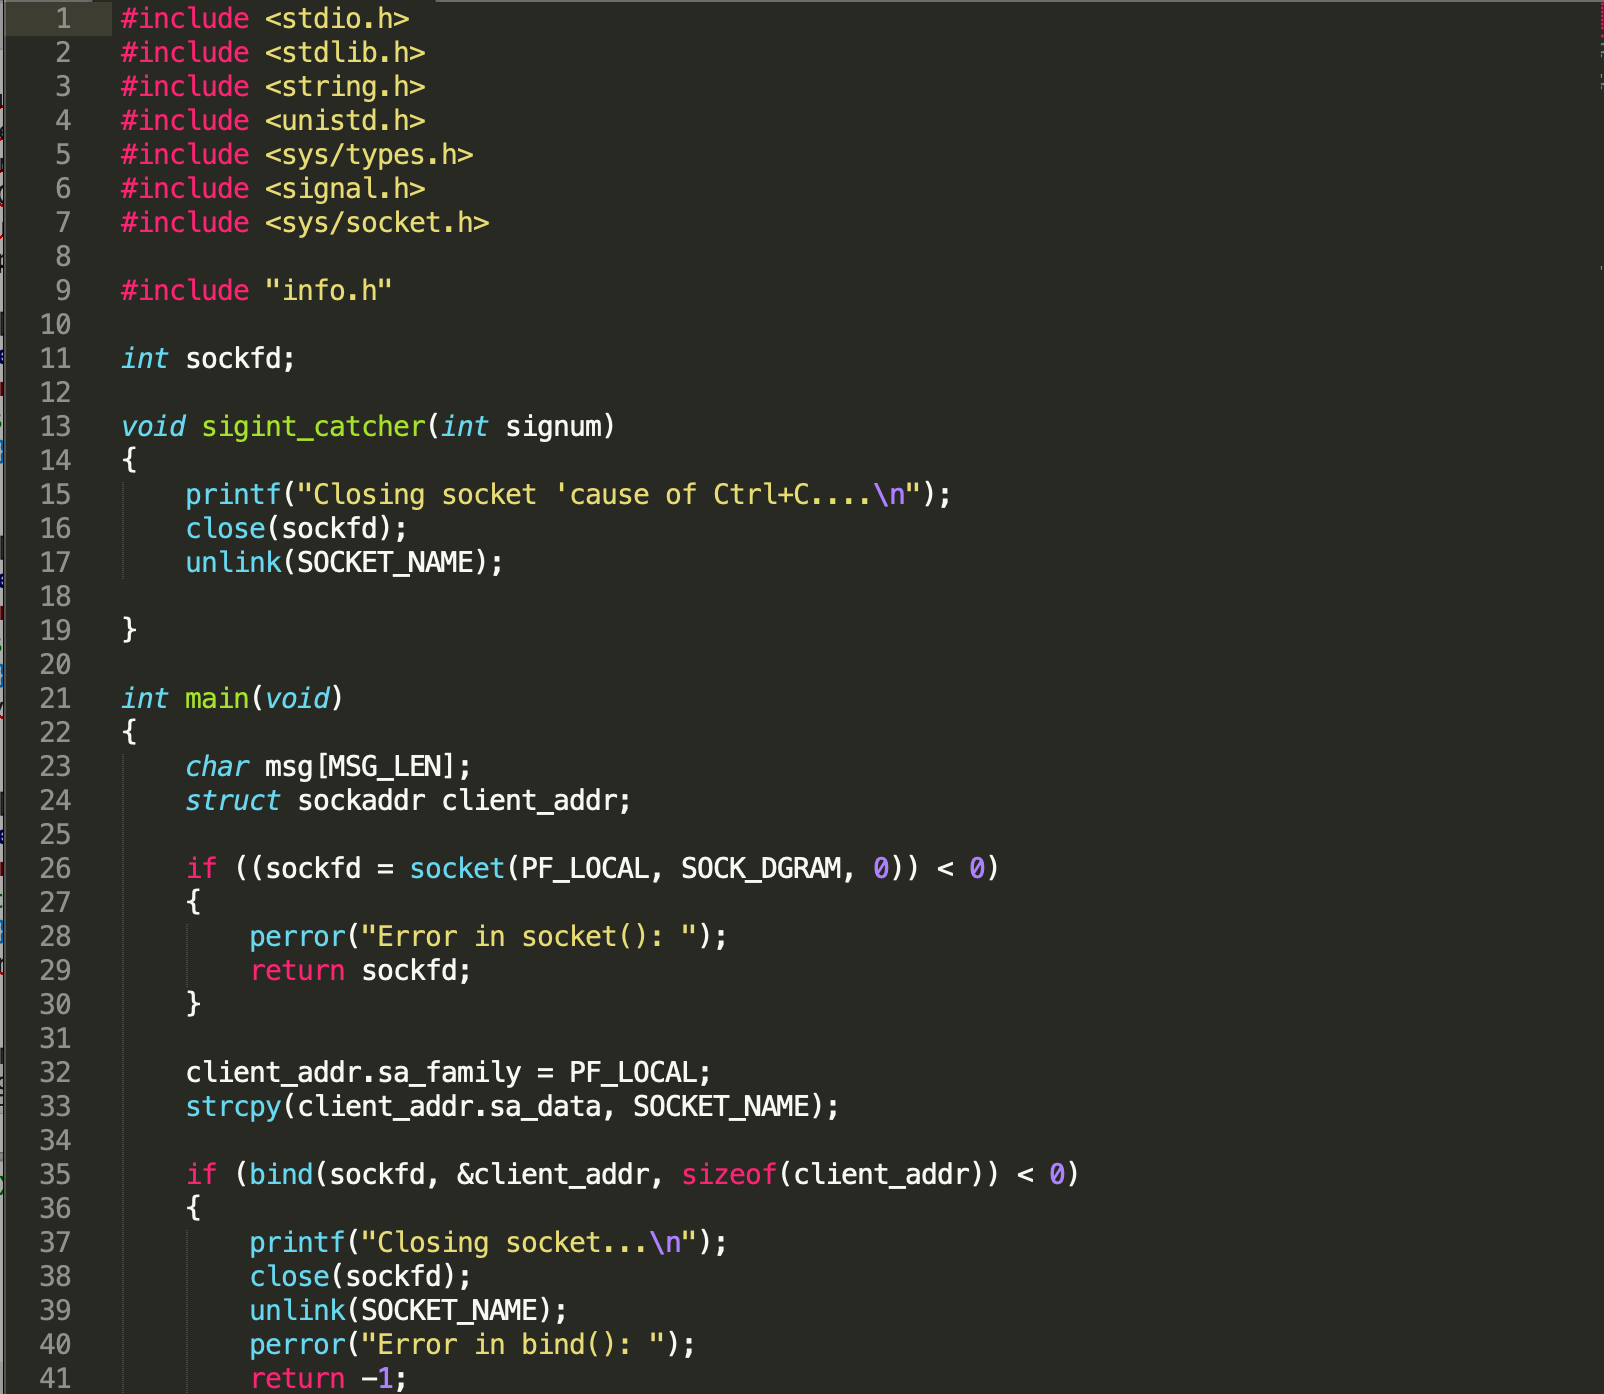
\includegraphics[scale = 0.6]{server1_1.png}}
			\label{ris:server1_1}
		\end{center}
	\end{figure}

	\newpage

	\begin{figure}[h!]
		\begin{center}
			{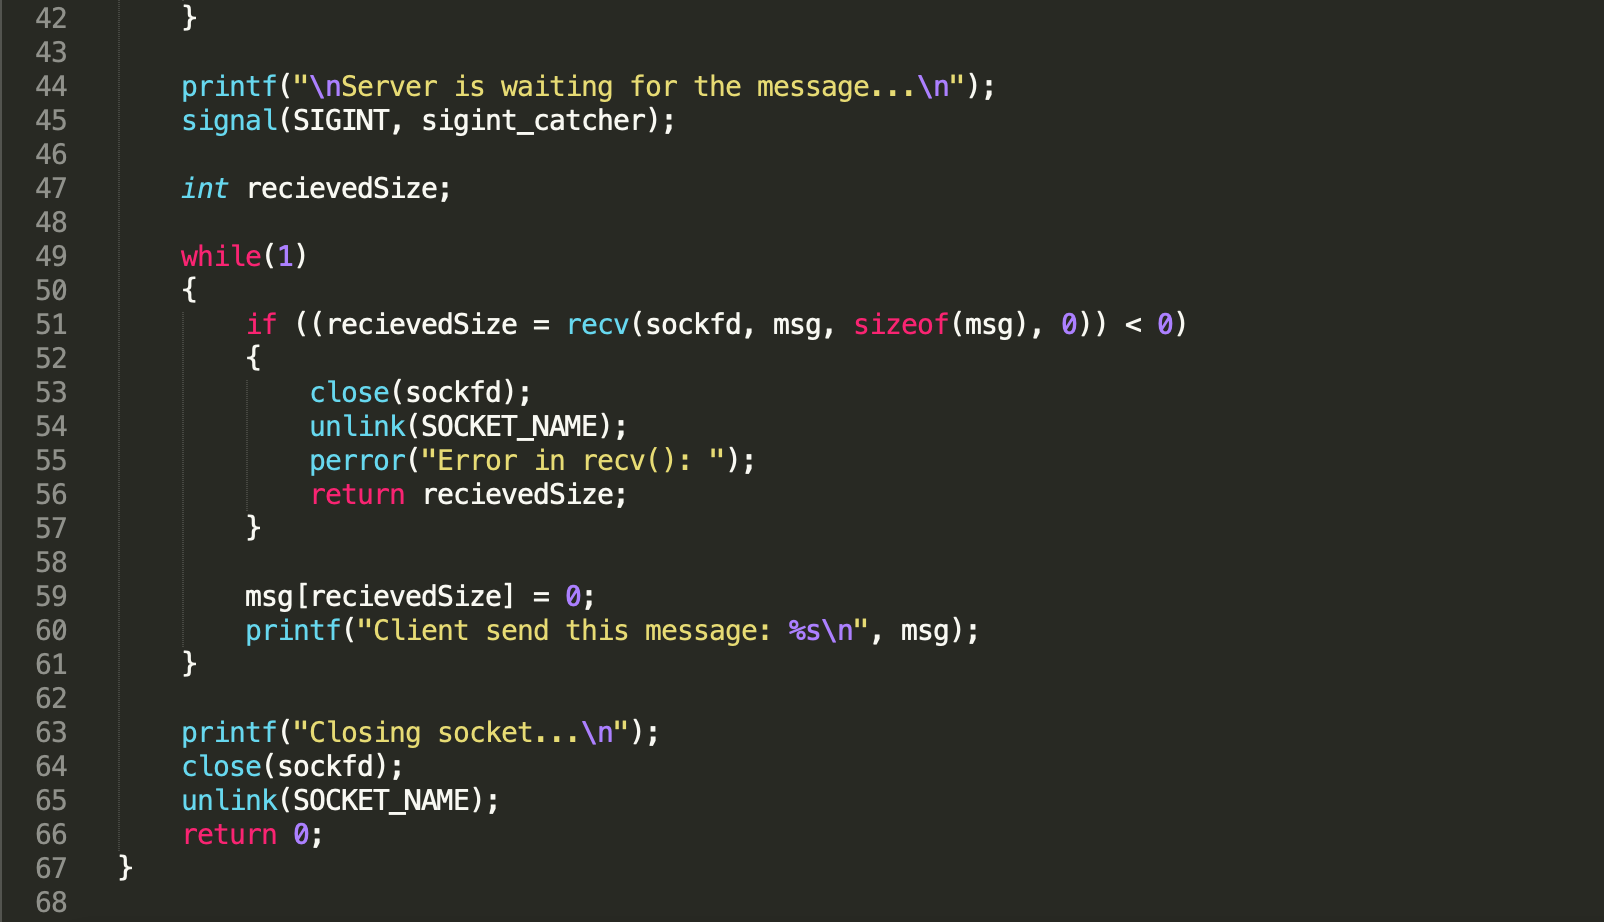
\includegraphics[scale = 0.6]{server2_1.png}}
			\label{ris:server2_1}
		\end{center}
		\caption{server.c}
	\end{figure}

	\begin{figure}[h!]
		\begin{center}
			{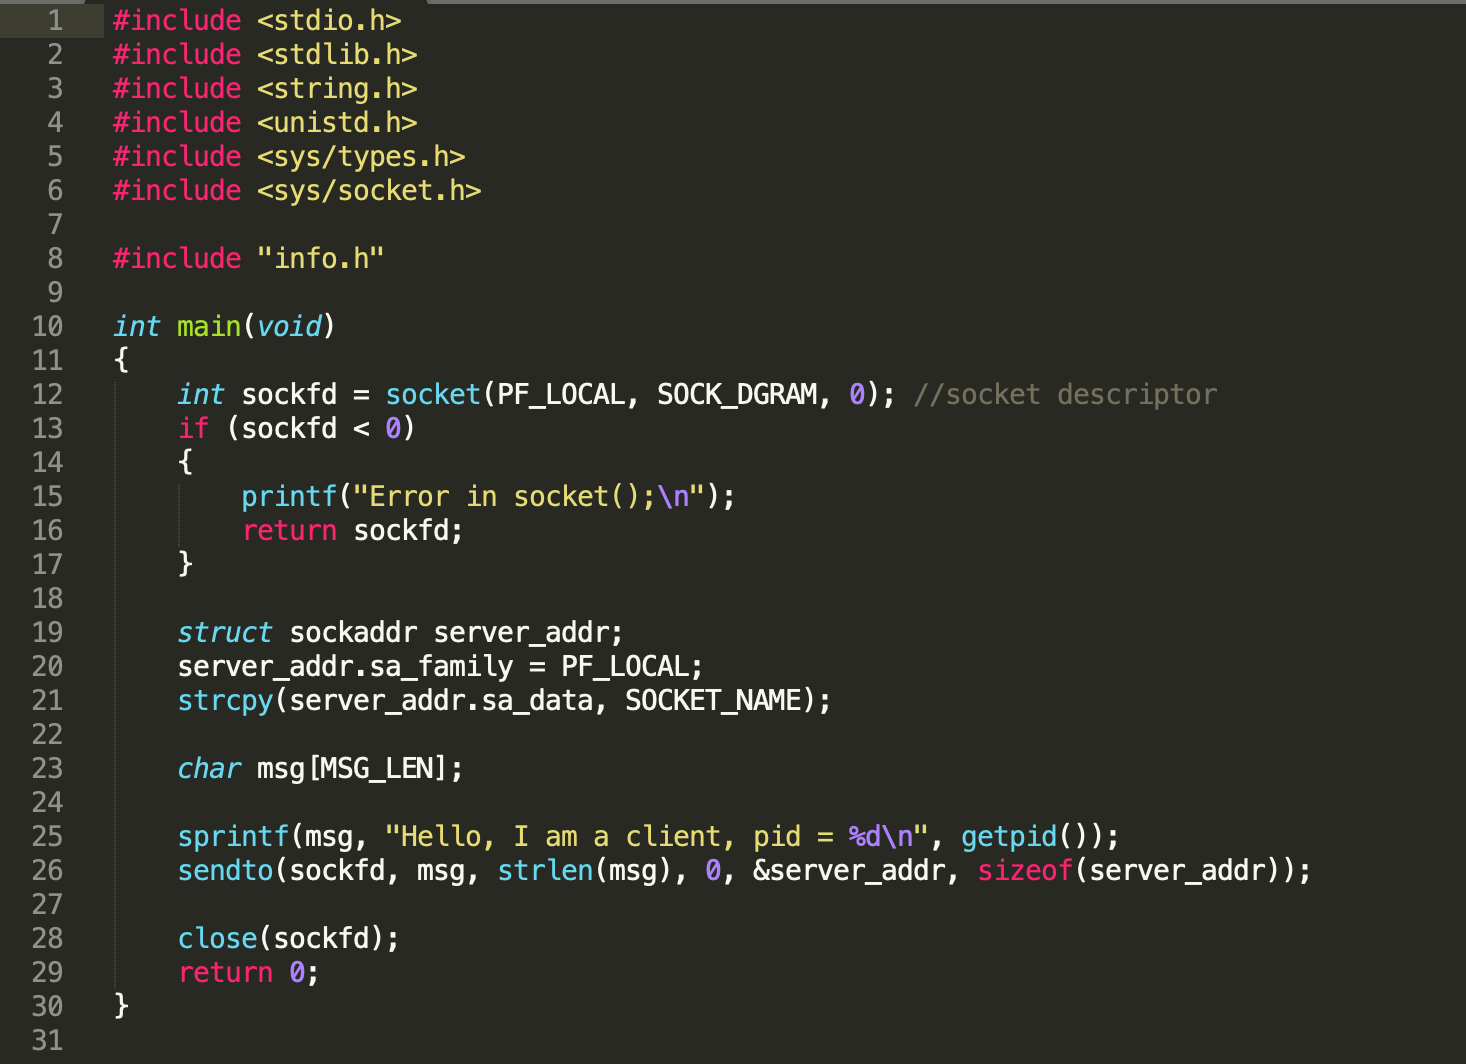
\includegraphics[scale = 0.6]{client_1.png}}
			\label{ris:client_1}
		\end{center}
		\caption{client.c}
	\end{figure}

	\begin{figure}[h!]
		\begin{center}
			{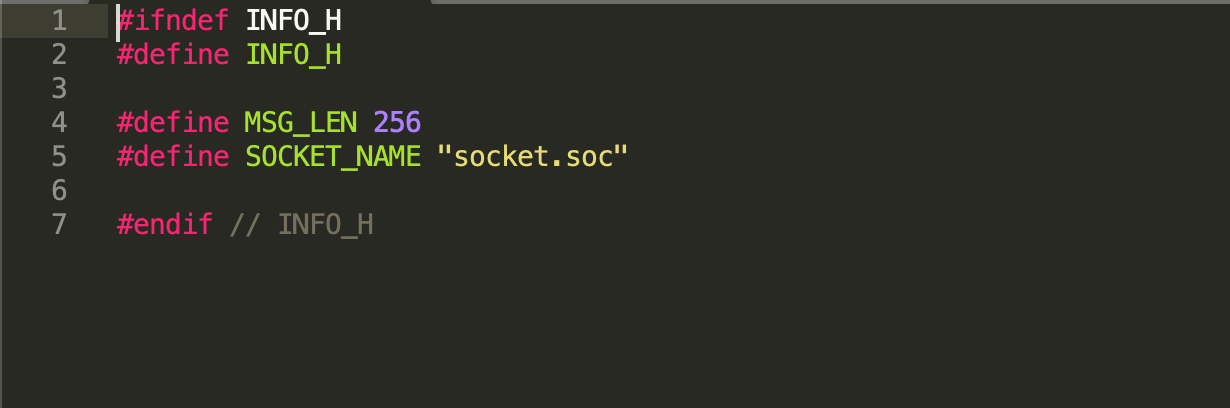
\includegraphics[scale = 0.6]{info_1.png}}
			\label{ris:info_1}
		\end{center}
		\caption{info.h}
	\end{figure}

	\subsection*{Демонстрация работы программы}
	
	Ниже представлены результаты работы программного комплекса с 5-ю запущенными клиентами. Выход из программы осуществляется сигналом SIGINT.
	
	\begin{figure}[h!]
		\begin{center}
			{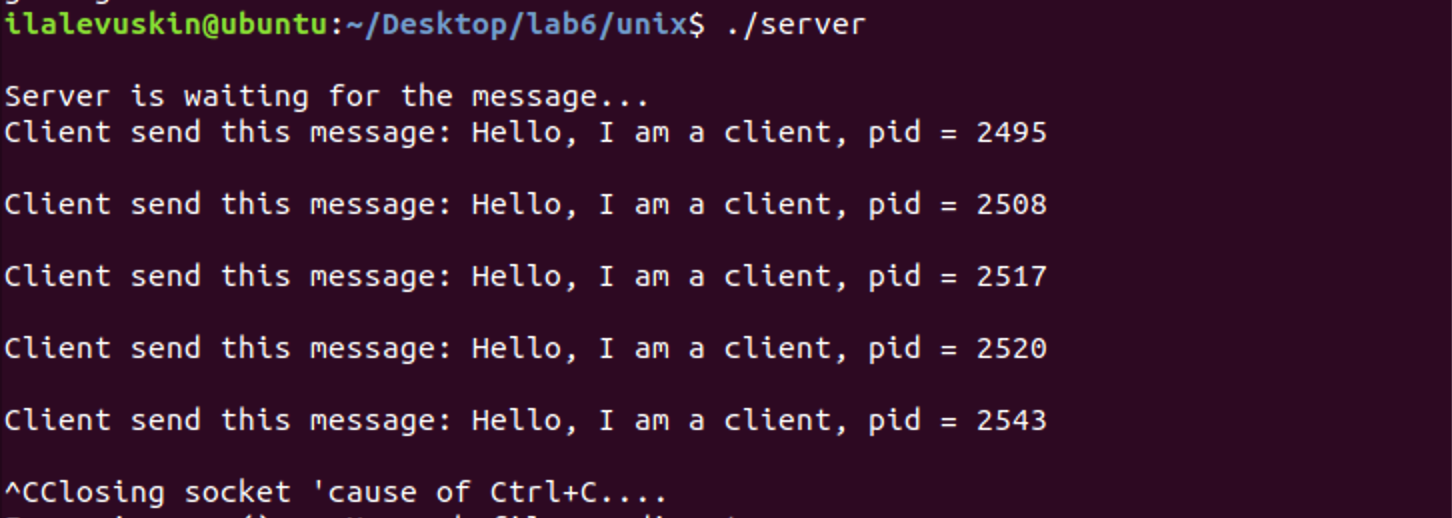
\includegraphics[scale = 0.7]{test_server_1.png}}
			\label{ris:test_server_1}
		\end{center}
	\end{figure}

	\begin{figure}[h!]
		\begin{center}
			{
\includegraphics[scale = 0.7]{test_client_1.png}}
			\label{ris:test_client_1}
		\end{center}
		\caption{Демонстрация работы программного комплекса}
	\end{figure}
	
	\newpage
	
	\section*{Задание 2.}
	
	{\bf Написать приложение по модели клиент-сервер, осуществляющее взаимодействие параллельных процессов, которые выполняются на разных компьютерах. Для взаимодействия с клиентами сервер должен использовать мультиплексирование. Сервер должен обслуживать запросы параллельно запущенных клиентов. При демонстрации работы программного комплекса необходимо запустить несколько клиентов (не меньше 5) и продемонстрировать, что сервер обрабатывает обращения каждого запущенного клиента.}
	
	Ниже приведен программный комплекс, реализующий поставленную задачу.
	
	\begin{figure}[h!]
		\begin{center}
			{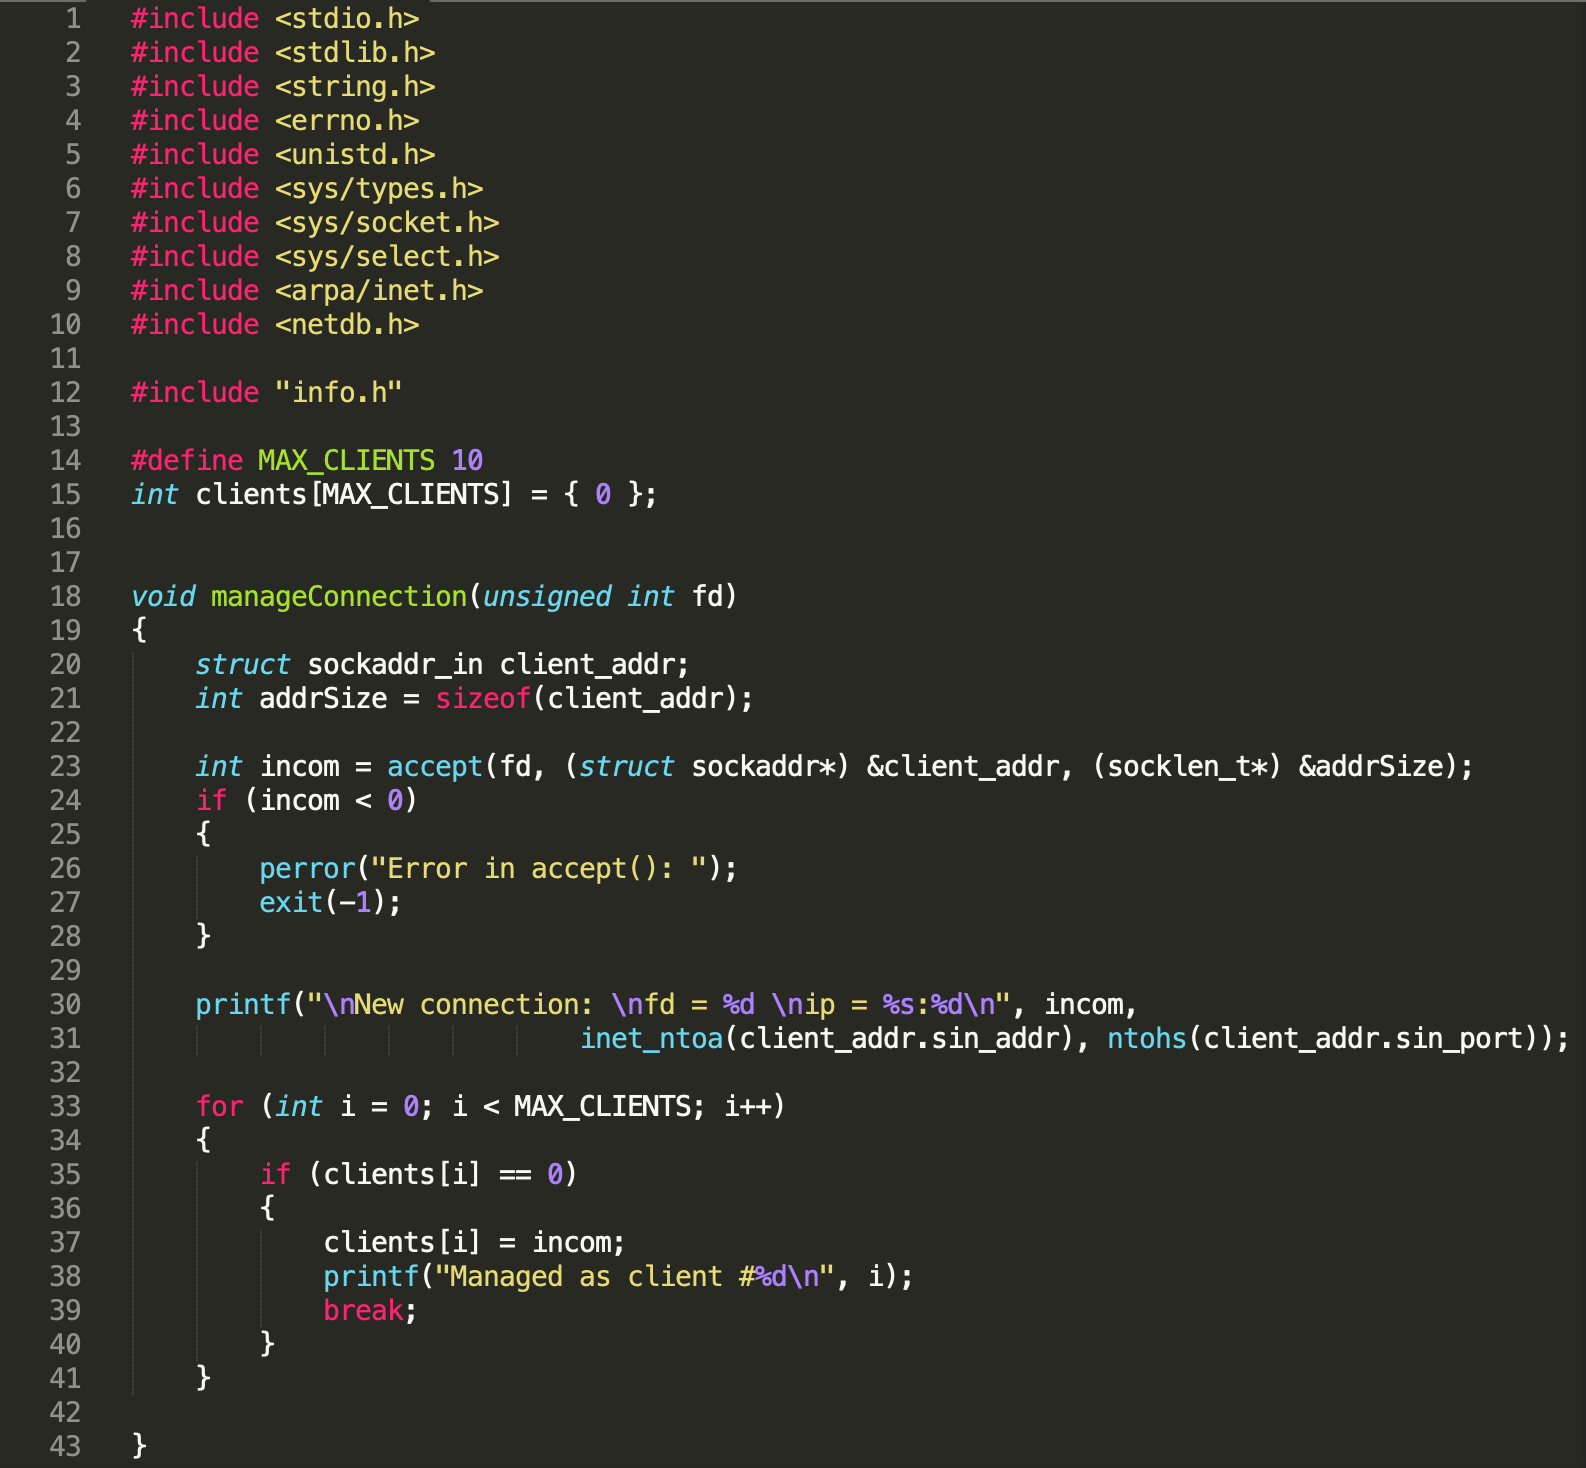
\includegraphics[scale = 0.6]{server1_2.png}}
			\label{ris:server1_2}
		\end{center}
		\caption{server.c}
	\end{figure}

	\newpage

	\begin{figure}[h!]
		\begin{center}
			{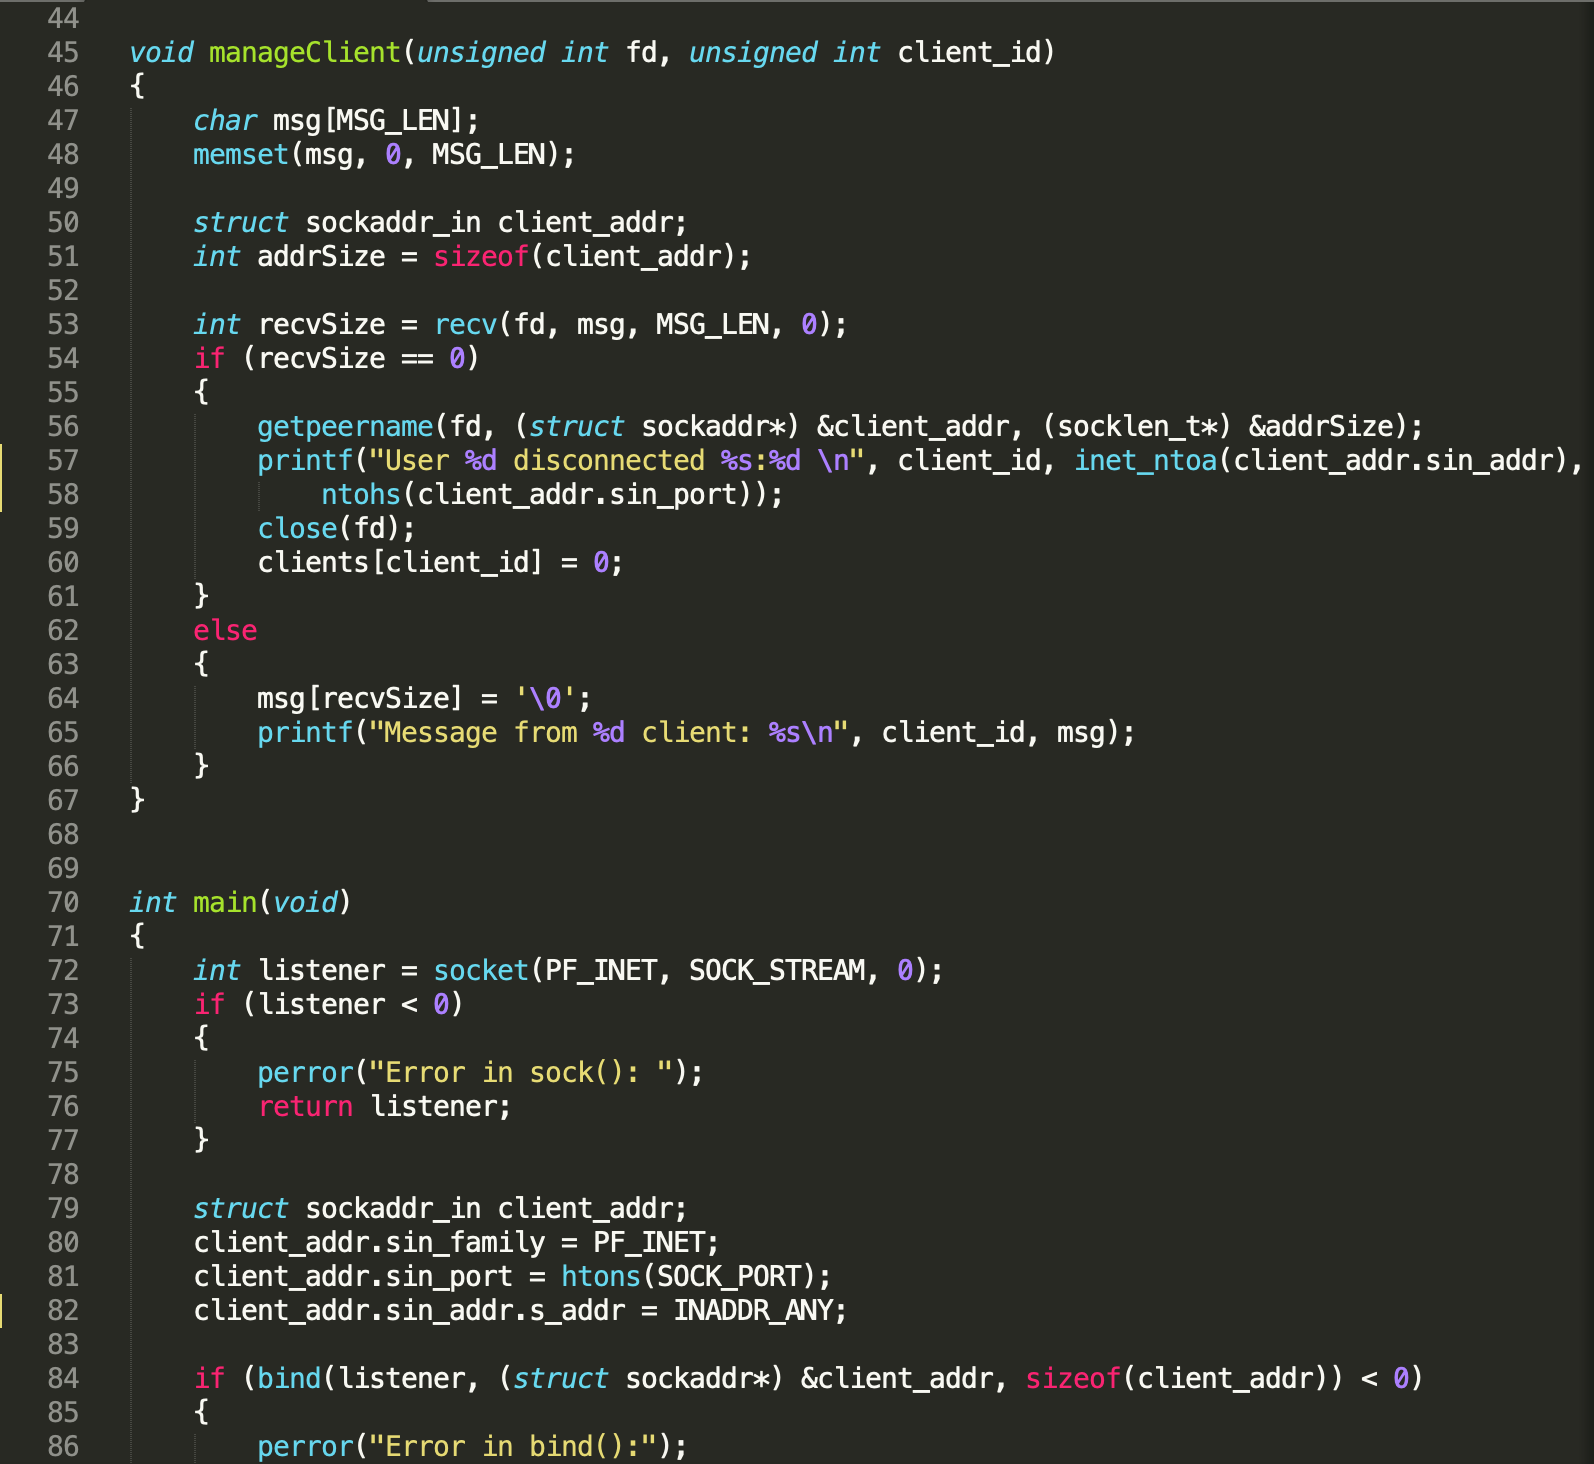
\includegraphics[scale = 0.6]{server2_2.png}}
			\label{ris:server2_2}
		\end{center}
		\caption{server.c}
	\end{figure}

	\newpage

	\begin{figure}[h!]
		\begin{center}
			{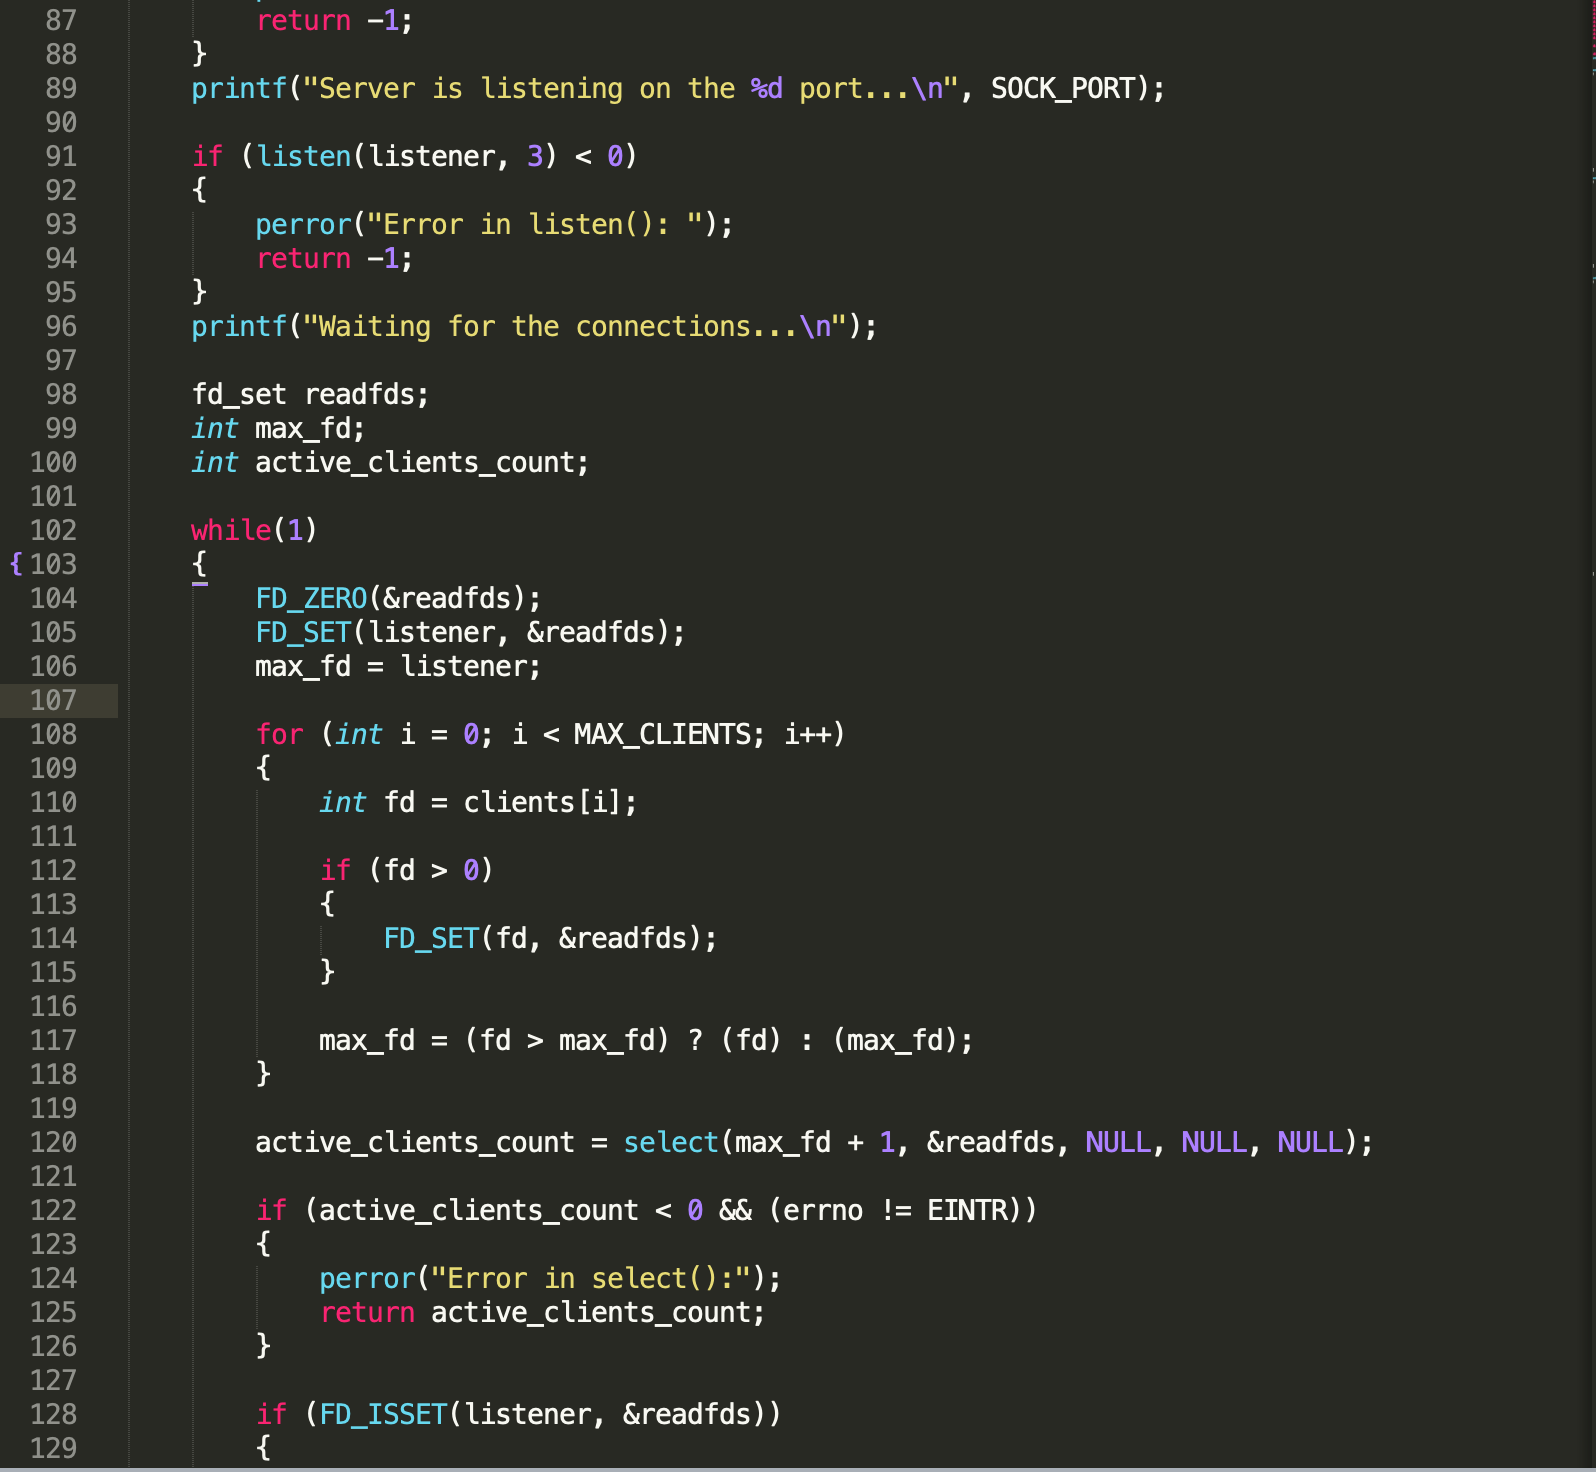
\includegraphics[scale = 0.6]{server3_2.png}}
			\label{ris:server3_2}
		\end{center}
		\caption{server.c}
	\end{figure}


	\begin{figure}[h!]
		\begin{center}
			{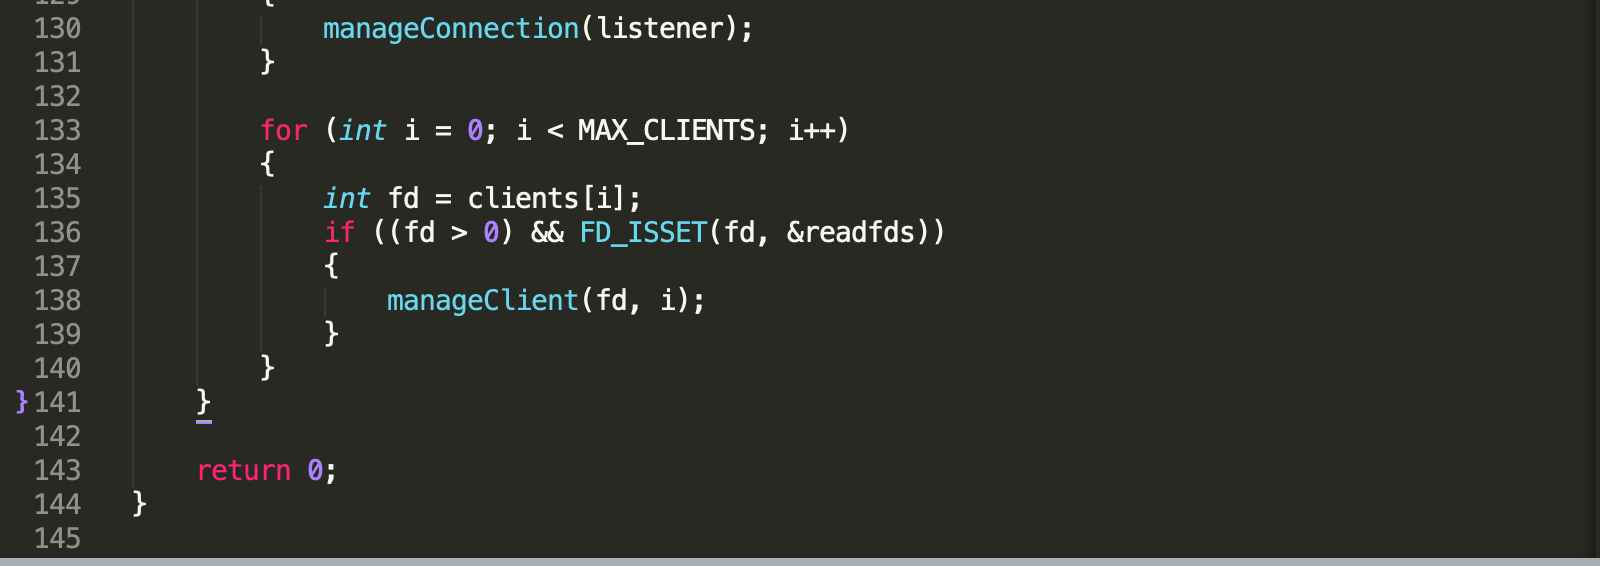
\includegraphics[scale = 0.6]{server4_2.png}}
			\label{ris:server4_2}
		\end{center}
		\caption{server.c}
	\end{figure}

	\newpage
	
	\begin{figure}[h!]
		\begin{center}
			{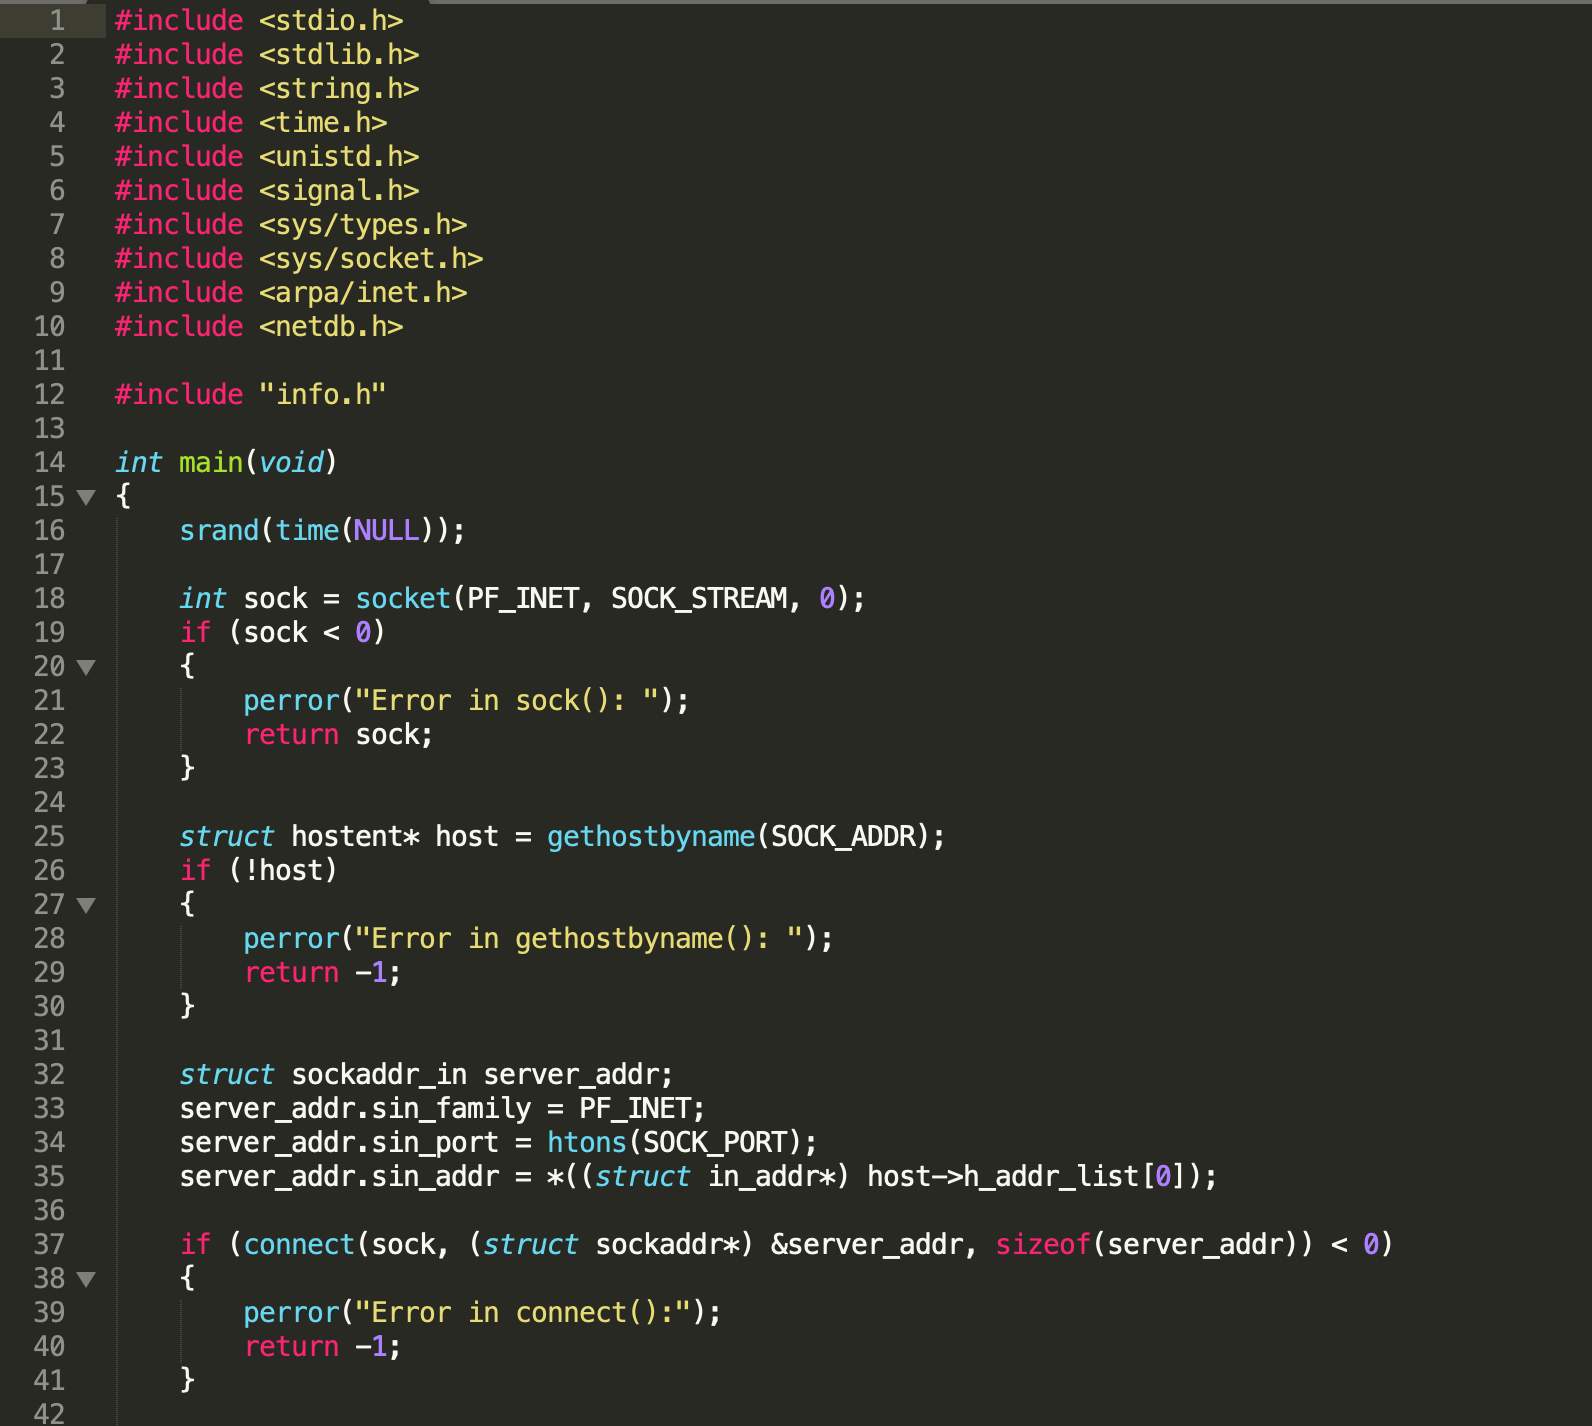
\includegraphics[scale = 0.55]{client1_2.png}}
			\label{ris:client_1_2}
		\end{center}
	\end{figure}

	\begin{figure}[h!]
		\begin{center}
			{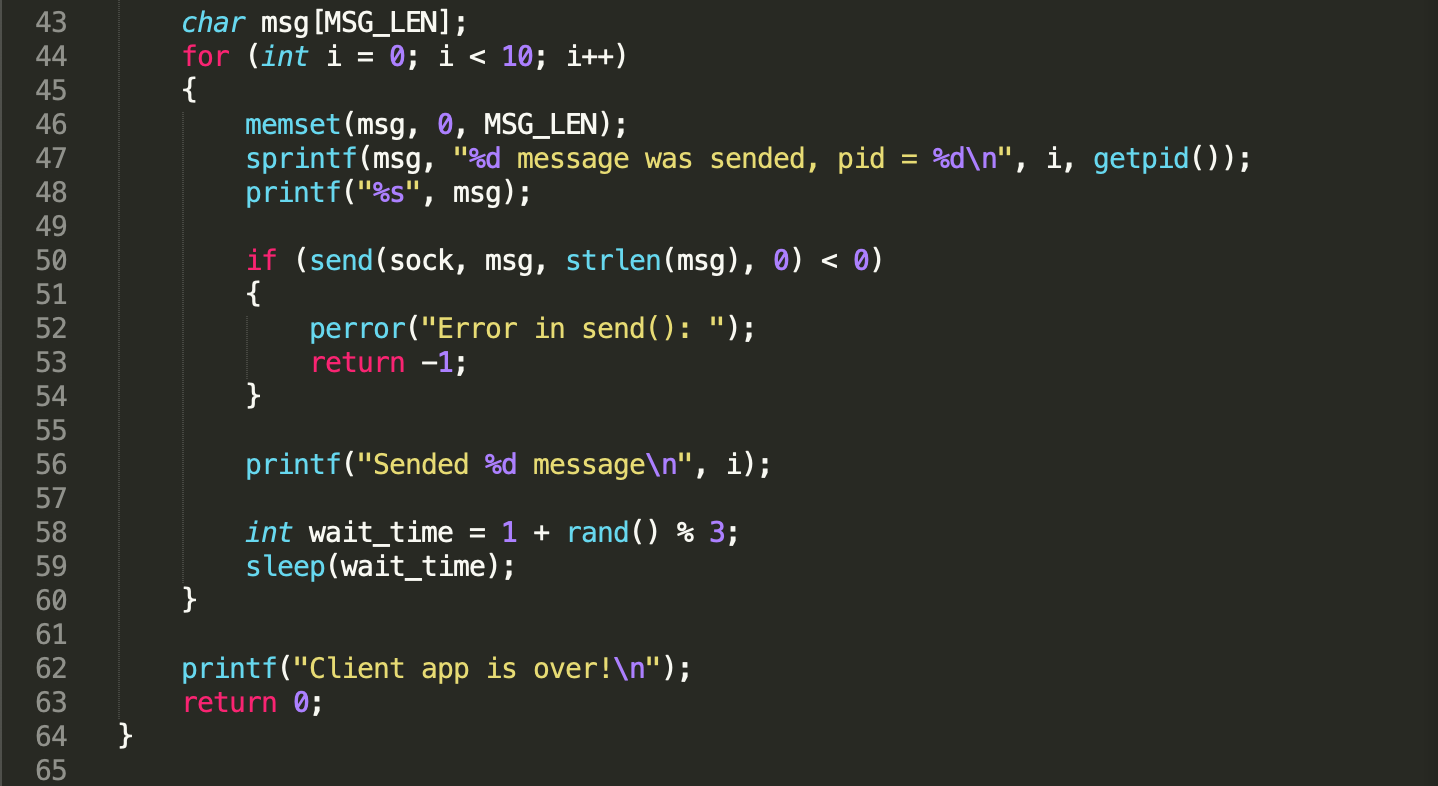
\includegraphics[scale = 0.6]{client2_2.png}}
			\label{ris:client_2_2}
		\end{center}
		\caption{client.c}
	\end{figure}

	\newpage
	
	\subsection*{Демонстрация работы программы}
	
	Ниже представлены результаты работы программного комплекса с 5-ю параллельно запущенными клиентами.
	
	\begin{figure}[h!]
		\begin{center}
			\begin{minipage}[h!]{0.5\linewidth}
				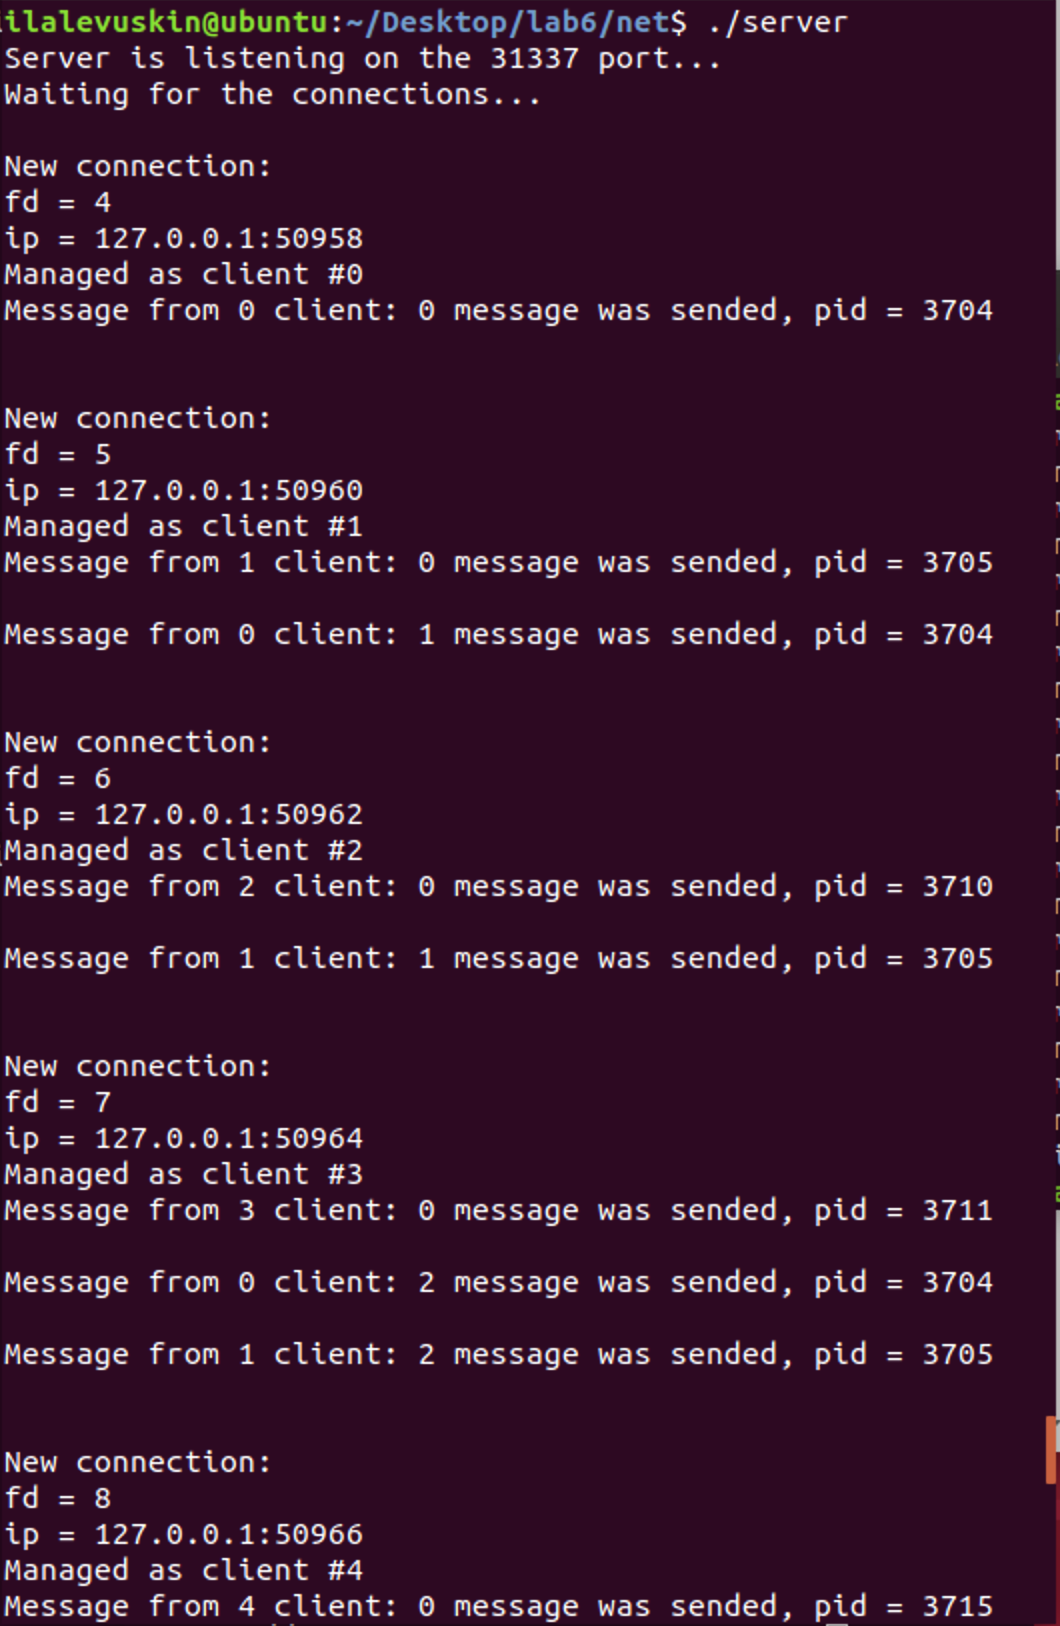
\includegraphics[width=1\linewidth]{test_server_1_2.png}
			\end{minipage}
			\begin{minipage}[h!]{0.49\linewidth}
				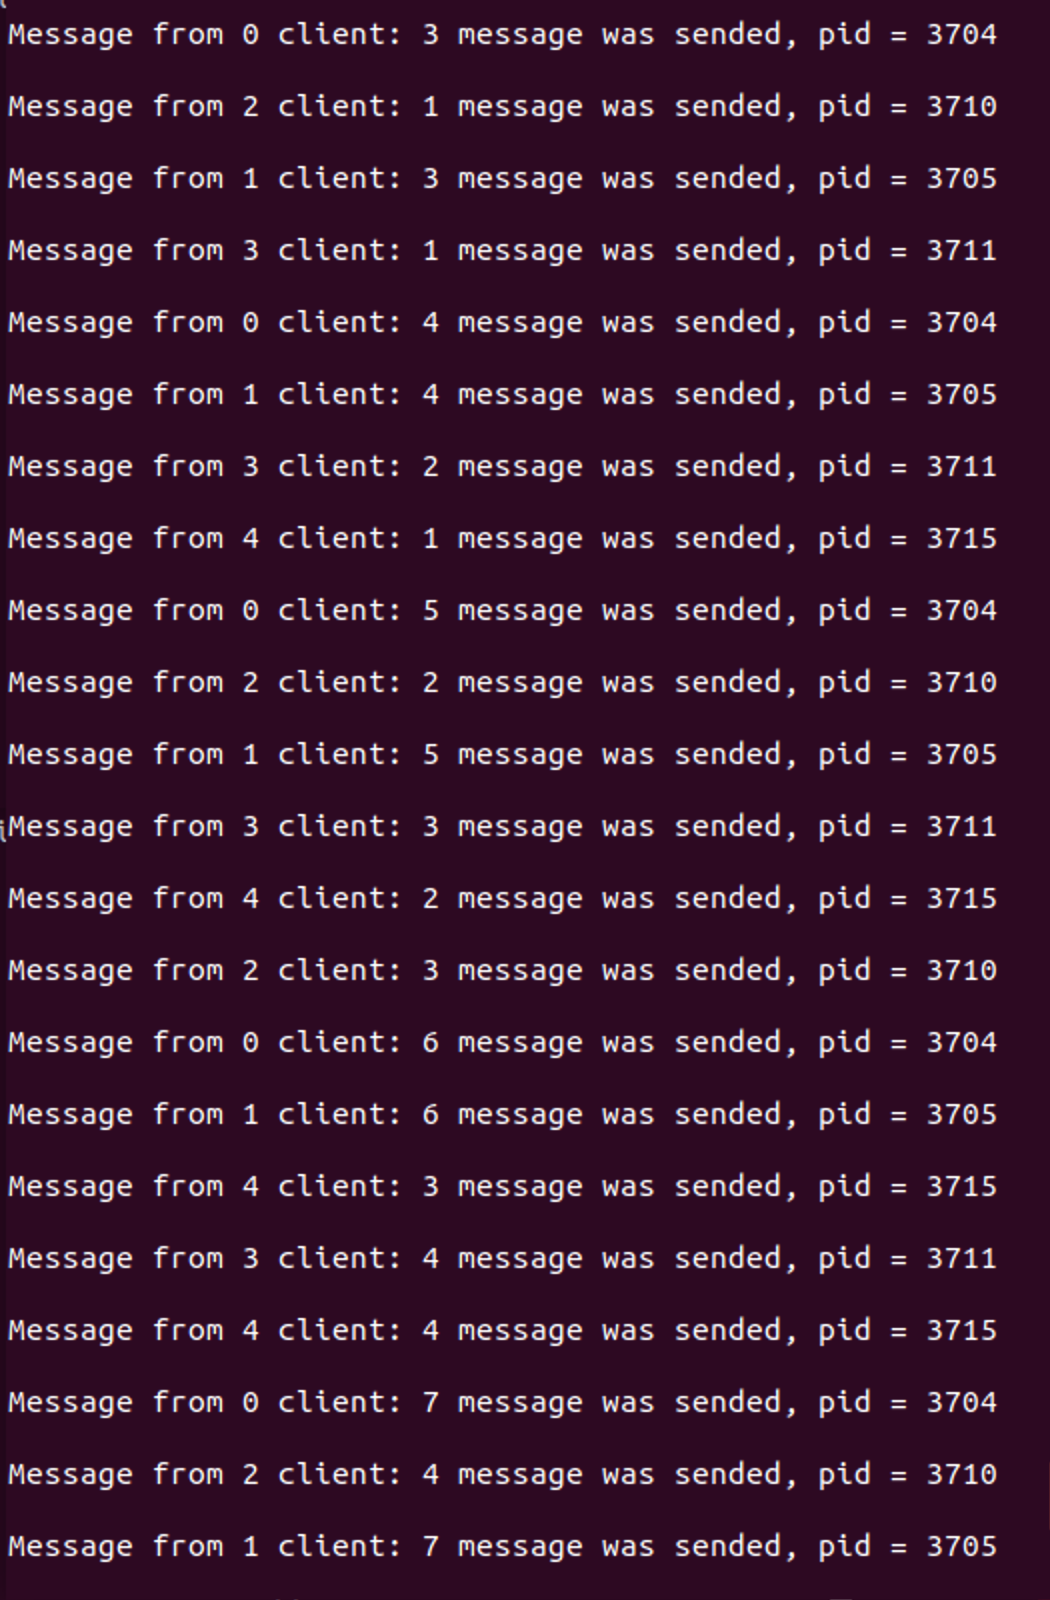
\includegraphics[width=1\linewidth]{test_server_2_2.png}
			\end{minipage}
			\label{ris:test_server_1_2}
			\caption{Результат работы сервера}
		\end{center}
	\end{figure}

	\begin{figure}[h!]
		\begin{center}
			{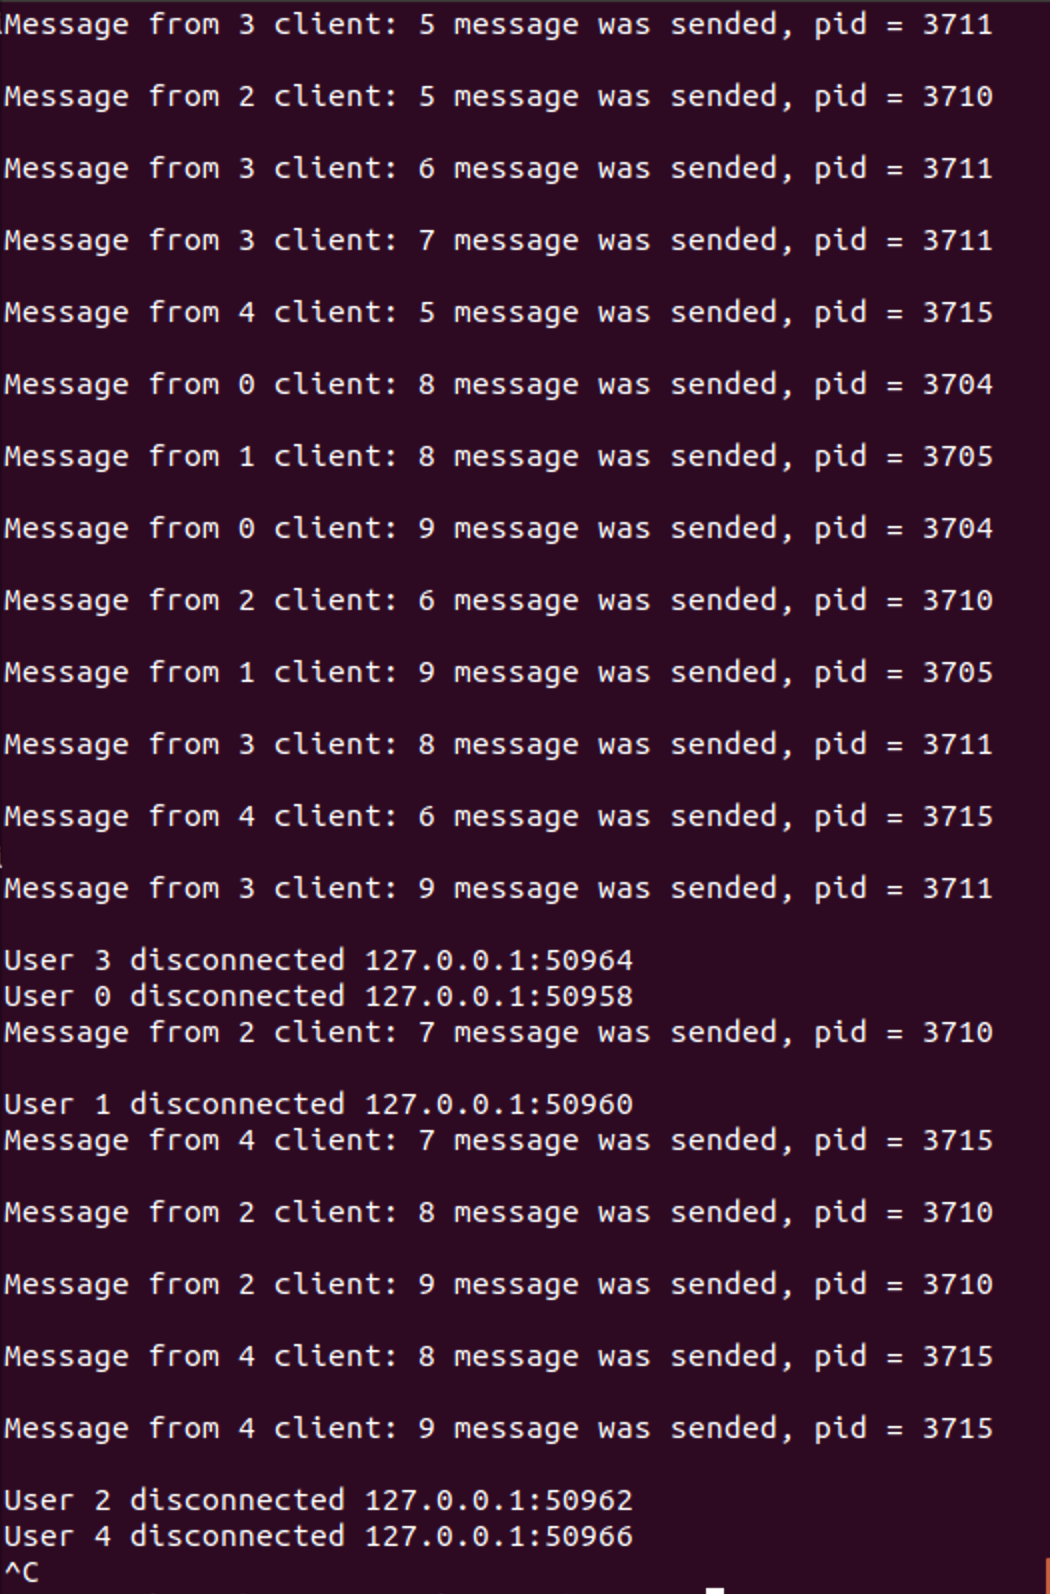
\includegraphics[scale = 0.7]{test_server_3_2.png}}
			\label{ris:test_server_3_2}
			\caption{Результат работы сервера}
		\end{center}
	\end{figure}

	\newpage

	\begin{figure}[h!]
		\begin{center}
			{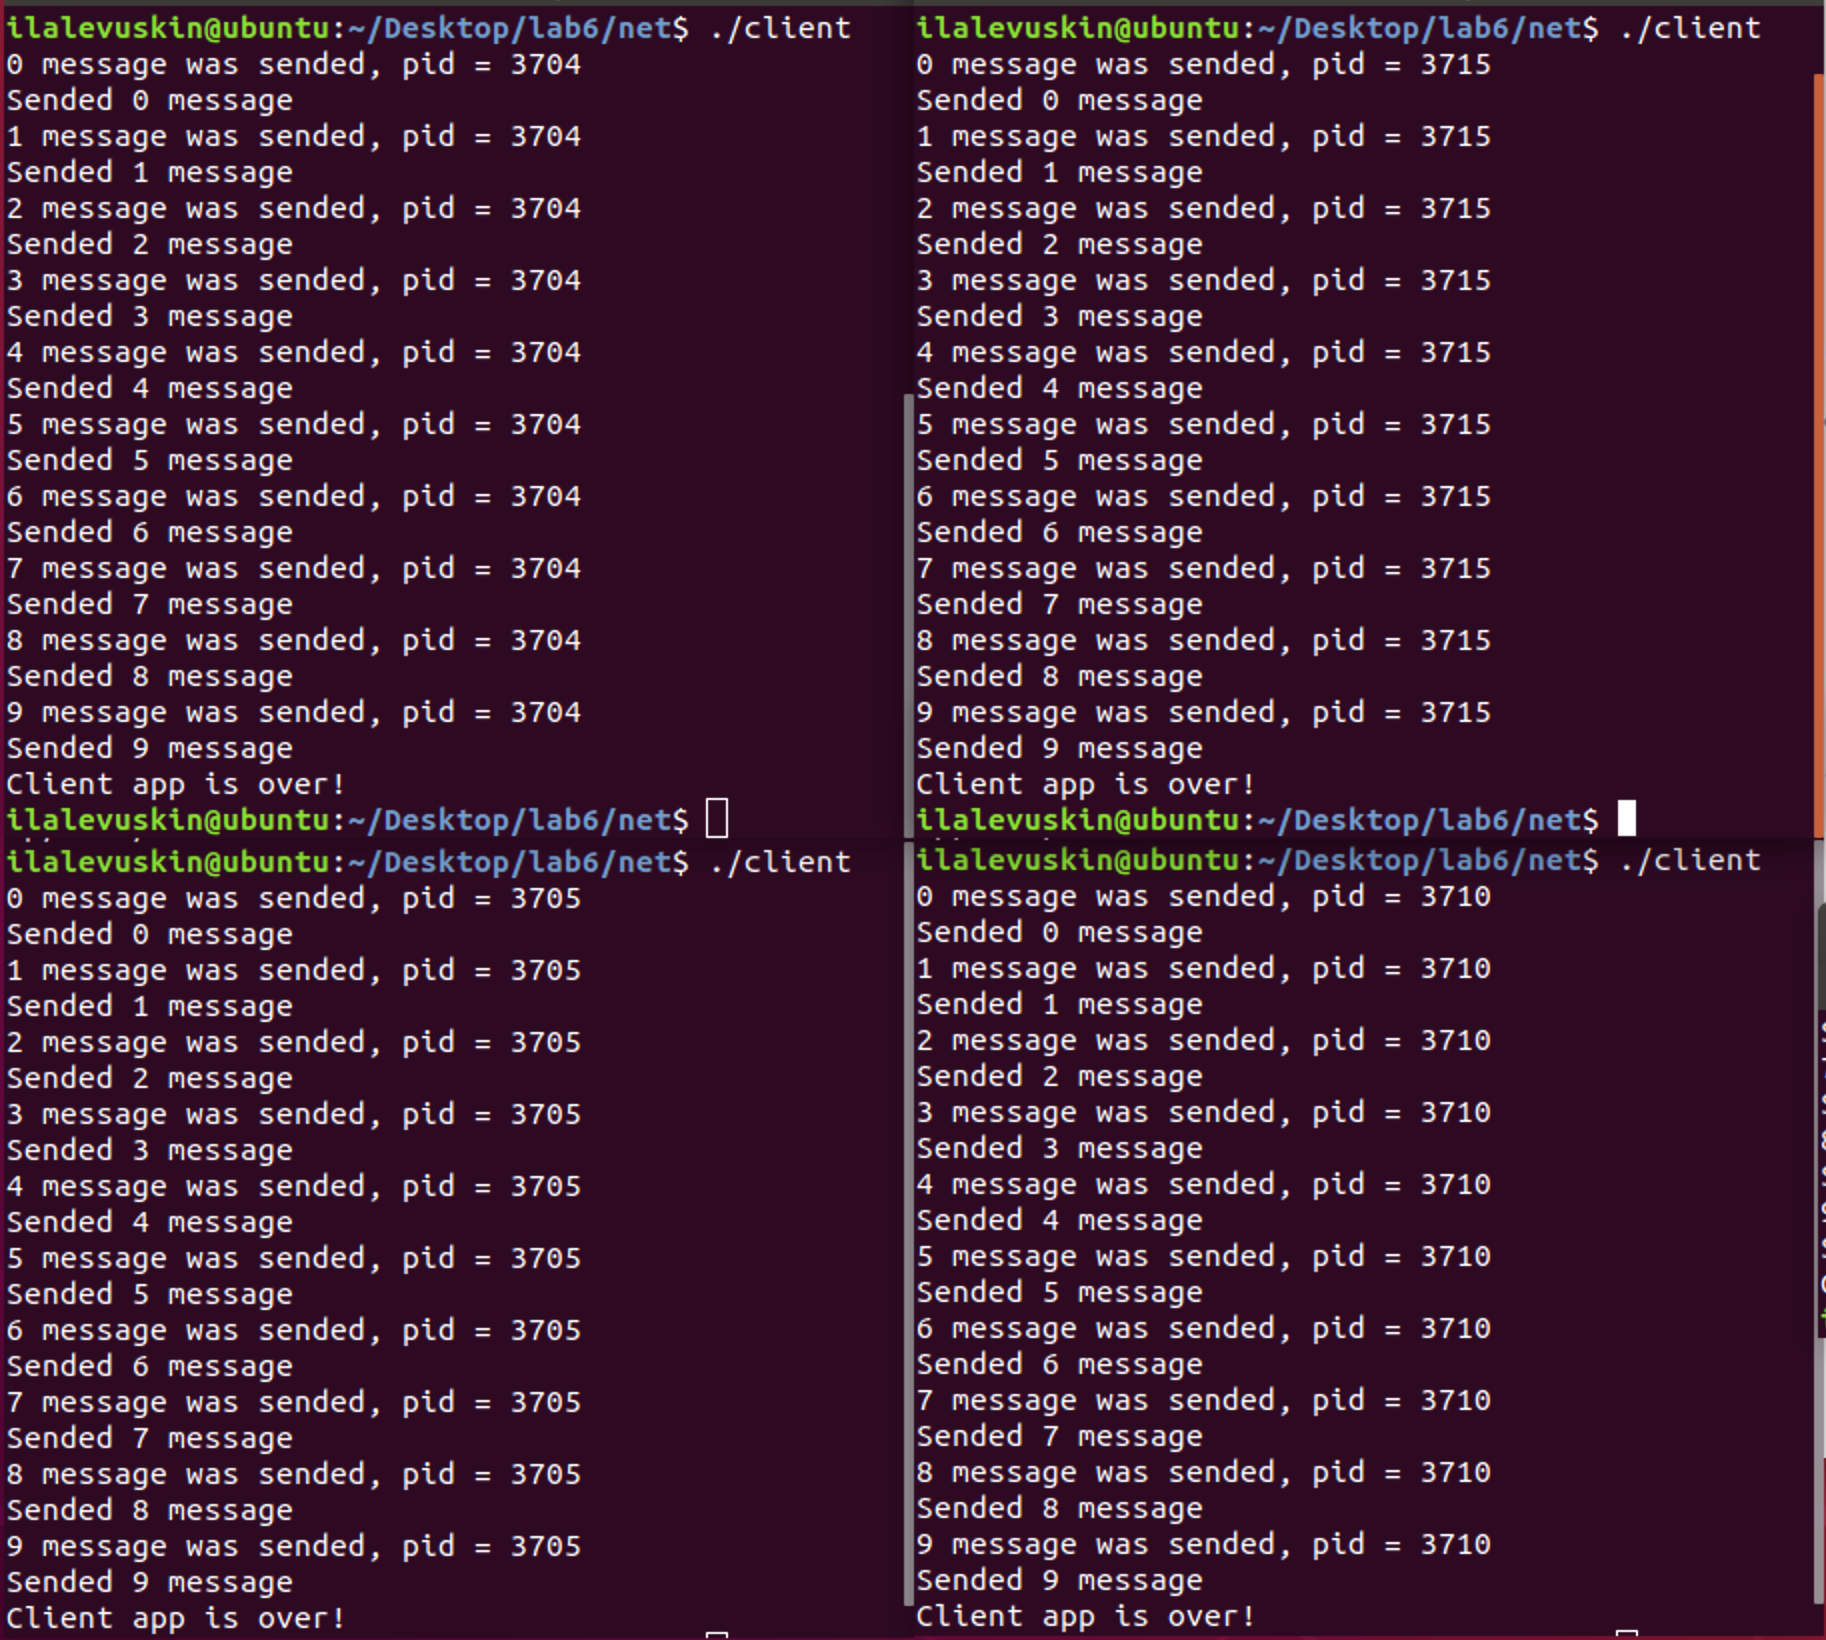
\includegraphics[scale = 0.5]{test_client_1_2.png}}
			\label{ris:test_client_1_2}
			\caption{Демонстрация запуска четырех клиентов}
		\end{center}
	\end{figure}
	
	\begin{figure}[h!]
		\begin{center}
			{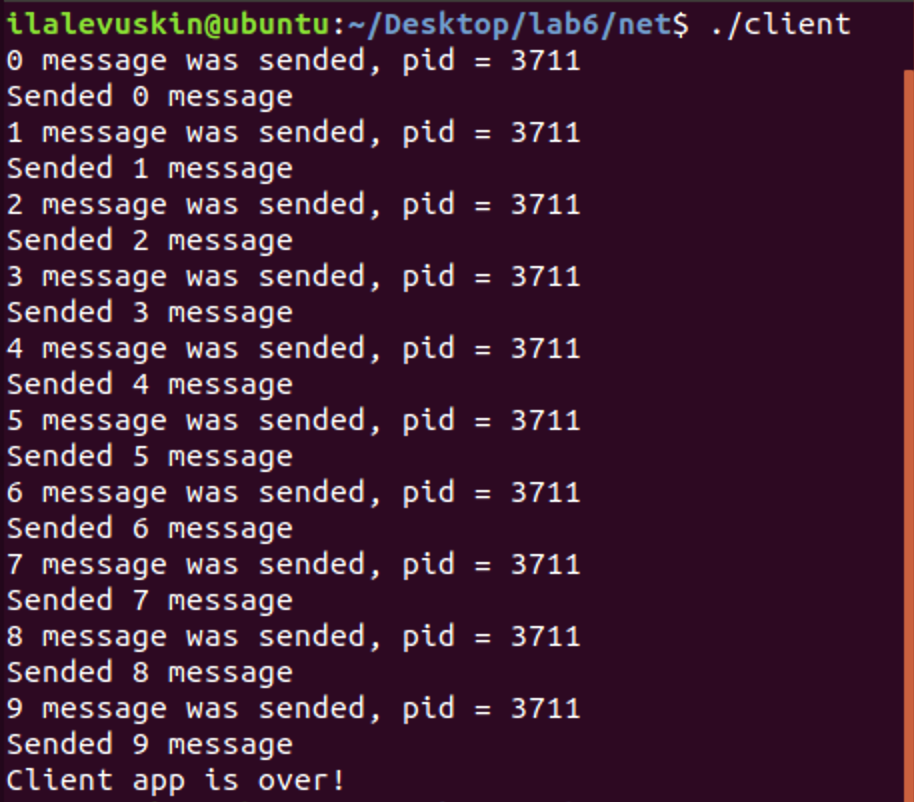
\includegraphics[scale = 0.7]{test_client_2_2.png}}
			\label{ris:test_client_2_2}
			\caption{Демонстрация запуска 5-ого клиента}
		\end{center}
	\end{figure}
	
\end{document}